% SafeRepair — IEEE Conference Paper Draft
% Template: \documentclass[conference]{IEEEtran}
% Target venue: ICCSAI 2026 / arXiv cs.SE
% Authors: Ammar Alam Khan, Amrit Singh Rawat, Aashay Sheware
% Dept. of Information Technology, Delhi Technological University

\documentclass[conference]{IEEEtran}
% \IEEEoverridecommandlockouts  % only needed for funding footnote; none here

\usepackage{cite}
\usepackage{amsmath,amssymb,amsfonts}
\usepackage{graphicx}
\usepackage{textcomp}
\usepackage{xcolor}
\usepackage{listings}
\usepackage{url}
\usepackage{dblfloatfix}
\usepackage{tikz}
\usetikzlibrary{arrows.meta,positioning,patterns}
\usepackage{pgfplots}
\pgfplotsset{compat=1.18}

\lstset{
  basicstyle=\ttfamily\fontsize{7}{8}\selectfont,
  language=C,
  breaklines=true,
  frame=single,
  captionpos=b,
  numbers=none,
  xleftmargin=3pt,
  xrightmargin=3pt,
  aboveskip=4pt,
  belowskip=3pt
}

\begin{document}

% ── Title ────────────────────────────────────────────────────────────────────

\title{SafeRepair: Deterministic, Static-Analysis-Guided\\
Repair of C Memory-Safety Vulnerabilities}

% ── Authors ──────────────────────────────────────────────────────────────────

\author{
\IEEEauthorblockN{Ammar Alam Khan}
\IEEEauthorblockA{\textit{Dept. of Information Technology}\\
\textit{Delhi Technological University}\\
New Delhi, India\\
ammaralamkhan\_it22a8\_53@dtu.ac.in}
\and
\IEEEauthorblockN{Amrit Singh Rawat}
\IEEEauthorblockA{\textit{Dept. of Information Technology}\\
\textit{Delhi Technological University}\\
New Delhi, India\\
amritsinghrawat\_it22a8\_54@dtu.ac.in}
\and
\IEEEauthorblockN{Aashay Sheware}
\IEEEauthorblockA{\textit{Dept. of Information Technology}\\
\textit{Delhi Technological University}\\
New Delhi, India\\
aashaysheware\_it22a8\_37@dtu.ac.in}
\and
\IEEEauthorblockN{Akshay Mool}
\IEEEauthorblockA{\textit{Assistant Professor, Dept. of Information Technology}\\
\textit{Delhi Technological University}\\
New Delhi, India\\
akshay.mool@dtu.ac.in}
}

\maketitle

% ── Abstract ─────────────────────────────────────────────────────────────────

\begin{abstract}
Buffer overflows, null pointer dereferences and improper memory management are
among the most exploited vulnerability classes in C software. Static analysis tools
can detect these patterns at scale but remediation remains a manual, per-alert
process. This paper presents SafeRepair, a rule-based automated program repair tool that
ingests static analysis alerts, confirms each vulnerability structurally against
the libclang abstract syntax tree and applies a deterministic source transformation.
Every patch is then validated with GCC compilation before being written. SafeRepair targets four CWE
patterns: suspicious realloc usage (CWE-401/690), missing null checks (CWE-690),
index-before-bounds-check (CWE-125/787) and unbounded sprintf (CWE-120). Evaluated
on 372 real-world alerts across 15 production open-source repositories spanning
editors, databases, game engines and network daemons, SafeRepair achieves 99.7\% repair accuracy on confirmed alerts with zero false positives. Requiring no training
data and producing deterministic output, SafeRepair is designed for deployment in
automated CI/CD pipelines where patch correctness cannot depend on human review.
\end{abstract}

\begin{IEEEkeywords}
automated program repair, static analysis, memory safety, C programming, CWE
\end{IEEEkeywords}

% ── I. Introduction ──────────────────────────────────────────────────────────

\section{Introduction}

Memory-safety bugs in C remain a leading cause of critical software vulnerabilities~\cite{b9}.
The NSA and CISA have explicitly recommended transitioning away from memory-unsafe
languages~\cite{b6} and patterns such as buffer overflows (CWE-120), out-of-bounds
access (CWE-125/787) and null pointer dereferences (CWE-690) collectively occupy
multiple entries in the annual CWE Top-25~\cite{b7}. Static analysis tools such as
clang-tidy and libclang can flag these patterns automatically across large codebases
but detection alone does not fix code. Developers must manually triage each alert
and apply straightforward but repetitive source transformations, a bottleneck that
allows known vulnerabilities to persist for months or years in production software.

Automated Program Repair (APR) research has taken several directions to close this
gap, from search-based tools such as GenProg~\cite{b8}, which guide genetic mutation
operators with a test suite, to template-based tools such as TBar~\cite{b10}, which
apply curated fix patterns when a structural match is confirmed.
Prophet~\cite{b11} sits between these categories: it learns a probabilistic model from
successful human patches and uses it to rank candidates in a generate-and-validate
loop for C programs. Learning-based tools achieve broad coverage: VulRepair~\cite{b4}
reports 43.7\% exact-match repair across diverse CVE types using a fine-tuned T5
model. VulMaster~\cite{b3} achieves 20.3\% exact match on 5,800 C/C++ vulnerable
functions. These learning-based methods
demand large training corpora and GPU infrastructure, produce non-deterministic
outputs that are difficult to audit and cannot provide formal assurance that a
generated patch is semantically correct. A 2025 survey of automated vulnerability
repair~\cite{b1} notes that template-based approaches perform well on specific
structurally-characterised vulnerability classes yet remain underrepresented
relative to learning-based methods despite their precision and auditability
advantages.

For vulnerability classes whose correct fix is fully determined by local abstract
syntax tree (AST) context, deterministic rule-based APR delivers properties that
probabilistic models cannot. The same input always produces the same output. Every
fix is a named, inspectable transformation with a documented reason. Zero false
positives are achievable by design because the handler either confirms the pattern
in the AST or declines to act. None of these guarantees are available from a model
that samples a repair from a learned distribution. SafeRepair does not compete
with neural APR on pattern breadth; it occupies a different point in the design
space where determinism and auditability matter more than generality.

This paper presents \textbf{SafeRepair}, a rule-based APR tool that realises these
properties across four well-characterised C memory-safety patterns. Evaluated on 372
alerts from 15 production repositories including SQLite, CPython, Vim, Netdata and
Radare2, SafeRepair achieves 99.7\% repair accuracy with zero false positives and no
training data requirement.

% ── II. Related Work ─────────────────────────────────────────────────────────

\section{Related Work}

APR approaches are broadly classified as search-based, template-based and
learning-based~\cite{b1}. Search-based tools such as GenProg~\cite{b8} generate
and validate candidate patches by applying genetic mutation operators and scoring
each candidate against a test suite. For security-focused repair, this test-suite dependency is a practical barrier:
tests that specifically exercise a buffer overflow or null dereference are seldom
written for production codebases, making search-based techniques impractical for
CWE-class memory-safety bugs.
Template-based tools such as TBar~\cite{b10} sidestep this by encoding known
fix patterns and applying them whenever a structural match is confirmed, achieving
high precision on well-characterised bug classes without any test-suite requirement.

Prophet~\cite{b11} falls between these two camps: it learns a probabilistic model
over patch operations from a corpus of successful human patches and uses it to rank
candidates in a generate-and-validate loop for C programs, producing correct patches
for 18 of 69 real-world defects. VulRepair~\cite{b4} advances this direction with
a fine-tuned T5 sequence-to-sequence model trained on CVE fix commits, reporting
43.7\% exact-match repair across diverse vulnerability types. VulMaster~\cite{b3}
further broadens the input representation to 5,800 C/C++ vulnerable functions,
reaching 20.3\% exact match. These approaches generalise well across diverse bug
types but none can produce deterministic, auditable output or carry formal
correctness arguments. They also require substantial GPU infrastructure and large
labelled training corpora.

The closest prior work to SafeRepair is Redemption by Svoboda et al.~\cite{b2},
a rule-based C/C++ APR tool driven by static analysis alerts from CodeSonar,
Fortify and Clang, covering null pointer dereferences, uninitialised reads and
dead-store patterns. Redemption achieves 94.4\% repair accuracy; however, that
result is reported on a single codebase across three analysers. SafeRepair targets
four memory-safety CWE patterns and is evaluated across 15 heterogeneous production
repositories, a substantially broader test corpus.

StaticFixer~\cite{b5} shares SafeRepair's static-analysis-guided pipeline
architecture, ingesting tool alerts and emitting verified source patches, but
targets JavaScript information-flow vulnerabilities and uses SMT-based condition
synthesis to construct the repair rather than AST pattern confirmation. Both tools
show that the static-analysis-to-repair pipeline is not specific to C or to any
one confirmation mechanism. A 2025 survey of automated vulnerability repair~\cite{b1}
identifies template-based and rule-based approaches as underrepresented relative
to learning-based methods despite their precision and auditability advantages.
Memory-safety bugs in C make a strong case for source-level repair: Szekeres
et al.~\cite{b9} document how buffer, heap and stack exploitation techniques have
persisted across decades, adapting to defensive mitigations such as ASLR and stack
canaries rather than disappearing. SafeRepair targets exactly this class of
persistent, structurally well-defined bugs with a deterministic, auditable pipeline
that none of the above systems provides.

% ── III. System Architecture ─────────────────────────────────────────────────

\section{System Architecture}
\label{sec:arch}

% ── Figure 1: Pipeline (two-column) ──────────────────────────────────────────
\begin{figure*}[t]
\centering
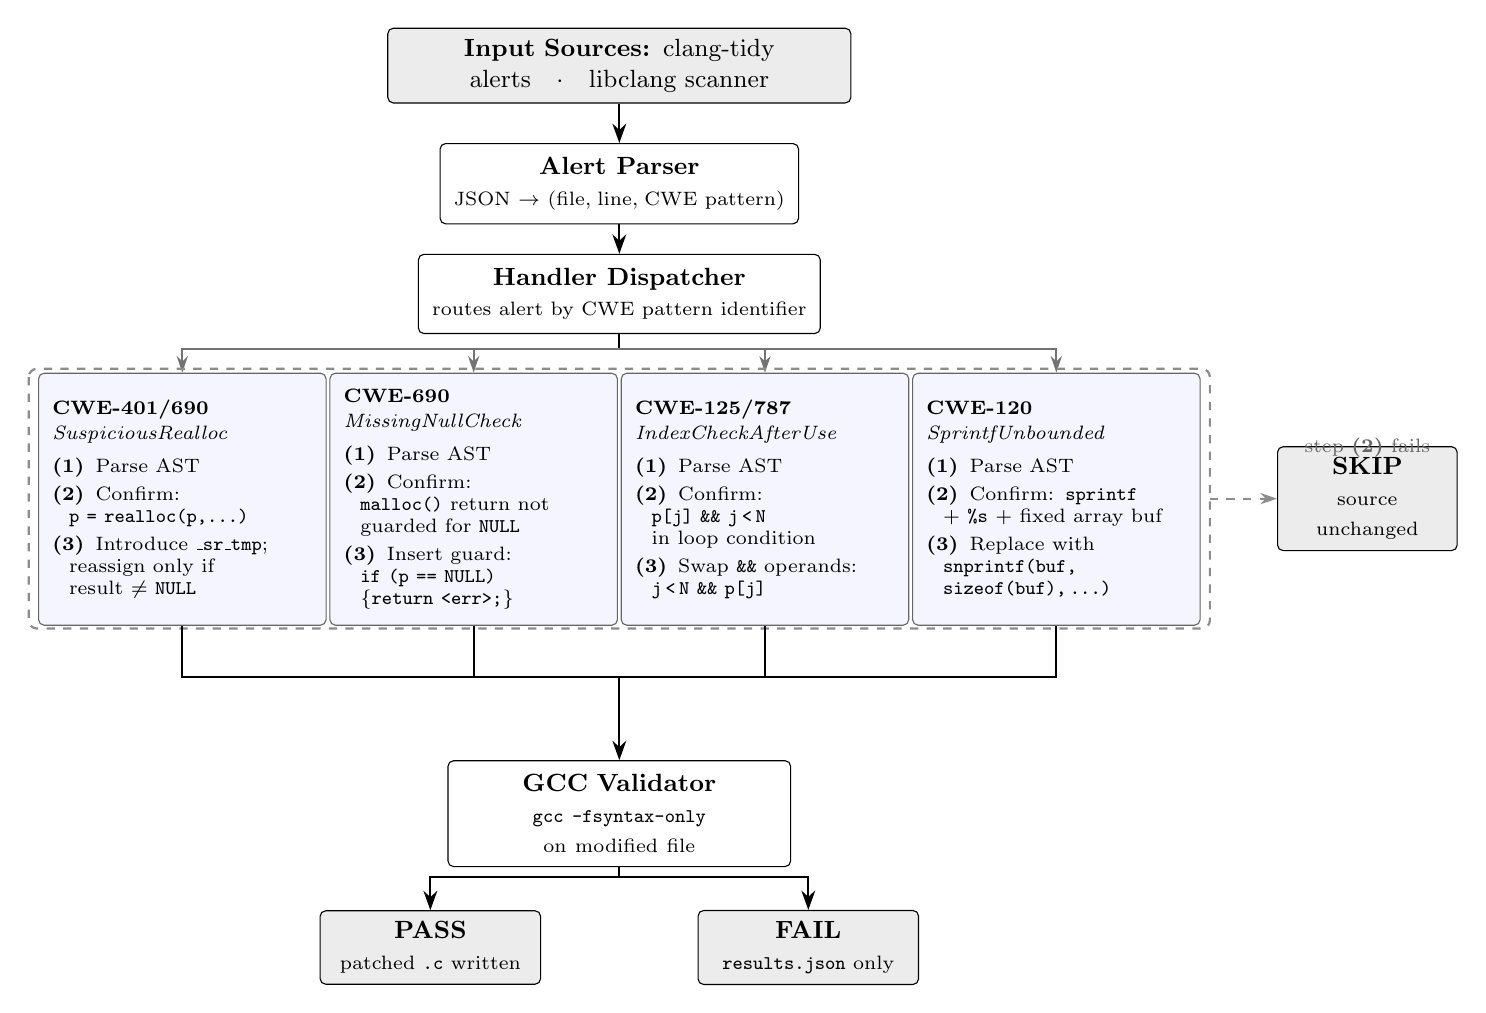
\begin{tikzpicture}[
  box/.style={rectangle, draw=black, rounded corners=2pt, fill=white,
              align=center, font=\small, inner sep=5pt,
              minimum width=3.0cm, minimum height=0.7cm},
  iobox/.style={rectangle, draw=black, fill=gray!15, rounded corners=2pt,
                align=center, font=\small, inner sep=4pt,
                minimum width=3.0cm, minimum height=0.6cm},
  hbox/.style={rectangle, draw=black!60, fill=blue!4, rounded corners=2pt,
               align=left, font=\scriptsize, inner sep=5pt,
               minimum width=3.6cm, minimum height=3.2cm,
               text width=3.3cm, anchor=north},
  arr/.style={-{Stealth[length=7pt,width=5pt]}, thick},
  darr/.style={-{Stealth[length=6pt,width=4pt]}, thick, draw=black!55},
  sarr/.style={-{Stealth[length=6pt,width=4pt]}, dashed, thick, draw=black!45},
]

%% Row 1 — Input
\node[iobox, minimum width=5.8cm, text width=5.6cm] (inp) at (0, 0) {%
  \textbf{Input Sources:}\enspace
  {\small clang-tidy alerts $\;\cdot\;$ libclang scanner}};

%% Row 2 — Alert Parser
\node[box] (parser) at (0, -1.5) {%
  \textbf{Alert Parser}\\
  {\scriptsize JSON $\to$ (file,\;line,\;CWE pattern)}};

%% Row 3 — Dispatcher
\node[box] (dispatch) at (0, -2.9) {%
  \textbf{Handler Dispatcher}\\
  {\scriptsize routes alert by CWE pattern identifier}};

%% Row 4 — 4 Handler boxes
%% Centers at x = -5.55, -1.85, +1.85, +5.55  (total handler row width = 14.7cm)
\node[hbox] (h1) at (-5.55, -3.9) {%
  \textbf{CWE-401/690}\\[1pt]%
  \textit{SuspiciousRealloc}\\[4pt]%
  \textbf{(1)}\enspace Parse AST\\[2pt]%
  \textbf{(2)}\enspace Confirm:\\%
  \hspace{6pt}\texttt{p = realloc(p,\ldots)}\\[2pt]%
  \textbf{(3)}\enspace Introduce \texttt{\_sr\_tmp};\\%
  \hspace{6pt}reassign only if\\%
  \hspace{6pt}result $\neq$ \texttt{NULL}};

\node[hbox] (h2) at (-1.85, -3.9) {%
  \textbf{CWE-690}\\[1pt]%
  \textit{MissingNullCheck}\\[4pt]%
  \textbf{(1)}\enspace Parse AST\\[2pt]%
  \textbf{(2)}\enspace Confirm:\\%
  \hspace{6pt}\texttt{malloc()} return not\\%
  \hspace{6pt}guarded for \texttt{NULL}\\[2pt]%
  \textbf{(3)}\enspace Insert guard:\\%
  \hspace{6pt}\texttt{if (p == NULL)}\\%
  \hspace{6pt}\texttt{\{return <err>;\}}};

\node[hbox] (h3) at (1.85, -3.9) {%
  \textbf{CWE-125/787}\\[1pt]%
  \textit{IndexCheckAfterUse}\\[4pt]%
  \textbf{(1)}\enspace Parse AST\\[2pt]%
  \textbf{(2)}\enspace Confirm:\\%
  \hspace{6pt}\texttt{p[j] \&\& j\,<\,N}\\%
  \hspace{6pt}in loop condition\\[2pt]%
  \textbf{(3)}\enspace Swap \texttt{\&\&} operands:\\%
  \hspace{6pt}\texttt{j\,<\,N \&\& p[j]}};

\node[hbox] (h4) at (5.55, -3.9) {%
  \textbf{CWE-120}\\[1pt]%
  \textit{SprintfUnbounded}\\[4pt]%
  \textbf{(1)}\enspace Parse AST\\[2pt]%
  \textbf{(2)}\enspace Confirm: \texttt{sprintf}\\%
  \hspace{6pt}$+$ \texttt{\%s} $+$ fixed array buf\\[2pt]%
  \textbf{(3)}\enspace Replace with\\%
  \hspace{6pt}\texttt{snprintf(buf,}\\%
  \hspace{6pt}\texttt{sizeof(buf),\,\ldots)}};

%% SKIP box: vertically centred on the handler row, to the right of all handlers
\node[iobox, minimum width=2.2cm, text width=2.0cm] (skipbox) at (9.5, -5.5) {%
  \textbf{SKIP}\\{\scriptsize source unchanged}};

%% Row 5 — GCC Validator  (hbus at -7.75; trunk = 1.4 cm to gcc.north at -9.15)
\node[box, minimum width=4.2cm, text width=4.0cm] (gcc) at (0, -9.5) {%
  \textbf{GCC Validator}\\
  {\scriptsize \texttt{gcc -fsyntax-only} on modified file}};

%% Row 6 — Outputs
\node[iobox, minimum width=2.8cm] (pass) at (-2.4, -11.2) {%
  \textbf{PASS}\\{\scriptsize patched \texttt{.c} written}};
\node[iobox, minimum width=2.8cm] (fail) at (2.4, -11.2) {%
  \textbf{FAIL}\\{\scriptsize \texttt{results.json} only}};

%% ── Arrows ─────────────────────────────────────────────────────────────────

\draw[arr] (inp) -- (parser);
\draw[arr] (parser) -- (dispatch);

%% Dispatch fan-out: one thick line from dispatch to junction, then one darr
%% arm per handler — no overlapping arrowheads on the shared segment
\coordinate (djct) at (0, -3.6);
\draw[thick] (dispatch.south) -- (djct);
\draw[darr] (djct) -| (h1.north);
\draw[darr] (djct) -| (h2.north);
\draw[darr] (djct) -| (h3.north);
\draw[darr] (djct) -| (h4.north);

%% Dashed bounding box around ALL four handler boxes — shows SKIP can exit
%% from any handler; avoids confusion with any one specific handler.
%% Box: x from -7.5 to 7.5 (h1 left edge ~-7.35, h4 right edge ~7.35),
%%      y from -3.85 (just above north anchors at -3.9) to -7.15 (just below
%%      south edges at -7.1).
\draw[dashed, black!45, thick, rounded corners=3pt]
  (-7.5,-3.85) rectangle (7.5,-7.15);

%% Handler fan-in to GCC: arms drop WITHOUT arrowheads to a shared bus at
%% y = -7.75 (0.65 cm below handler south at -7.1), then ONE trunk arrow
%% runs from the bus centre to gcc.north — single clean arrowhead.
\coordinate (hbus) at (0, -7.75);
\draw[thick] (h1.south) -- ++(0,-0.65) -| (hbus);
\draw[thick] (h2.south) -- ++(0,-0.65) -| (hbus);
\draw[thick] (h3.south) -- ++(0,-0.65) -| (hbus);
\draw[thick] (h4.south) -- ++(0,-0.65) -| (hbus);
\draw[arr] (hbus) -- (gcc.north);

%% SKIP: horizontal dashed arrow from bounding box right edge to SKIP box.
%% Label sits above the SKIP box (y=-4.85), clear of both the arrow and the box.
\draw[sarr] (7.5,-5.5) -- (skipbox.west);
\node[font=\scriptsize, text=black!60] at (9.5,-4.85)
  {step \textbf{(2)} fails};

%% GCC fan-out: one thick line to junction, then one arr arm per output node
\coordinate (gjct) at (0,-10.3);
\draw[thick] (gcc.south) -- (gjct);
\draw[arr] (gjct) -| (pass.north);
\draw[arr] (gjct) -| (fail.north);

\end{tikzpicture}
\caption{SafeRepair pipeline architecture. Alerts are routed by CWE pattern to one
of four handlers. Each handler (1)~parses the file AST with libclang, (2)~confirms
the vulnerability structure and (3)~applies the source transformation. If step~(2)
fails the alert is marked \textbf{SKIP} and no file is modified. Validated patches
are classified as \textbf{PASS} or \textbf{FAIL}.}
\label{fig:pipeline}
\end{figure*}
% ─────────────────────────────────────────────────────────────────────────────

Fig.~\ref{fig:pipeline} shows the SafeRepair pipeline. It comprises three stages:
alert ingestion, handler dispatch and GCC validation.

\subsection{Alert Ingestion}
The alert parser (\texttt{alert\_parser.py}) reads structured JSON produced by
clang-tidy or the custom libclang scanner, extracting the file path, line number
and pattern identifier for each alert. Alerts from multiple scanners are normalised
to the same internal format before being passed to the dispatcher.

\subsection{Handler Dispatch}
The pipeline (\texttt{pipeline.py}) routes each alert to the corresponding handler
by pattern identifier. The handler invokes libclang to parse the target file,
navigates the AST to the flagged location and applies the transformation only if
the expected vulnerability structure is confirmed. If the AST does not match the
expected pattern, whether because of a macro expansion, an interprocedural
reference or a previously applied fix, the handler returns \texttt{None} and the
alert is marked \textbf{SKIP} with the source file left unchanged.

\subsection{GCC Validation}
After a handler produces a candidate patch, \texttt{validator.py} runs
\texttt{gcc -fsyntax-only} on the modified file. A patch is marked \textbf{PASS}
if this succeeds and \textbf{FAIL} if a syntax error is introduced. Because each
transformation preserves syntactic validity by construction, the GCC step acts as
an independent safety check rather than the primary correctness mechanism.

\subsection{Right-or-Silent Design Principle}
Every handler is written to be correct or to abstain. No handler infers from
incomplete context or applies a transformation it cannot verify against the AST.
Zero false positives follow directly from this conservatism: the tool is either
provably right or produces no output. A skipped alert leaves the source
file byte-for-byte identical to its original state.

% ── IV. Pattern Handlers ─────────────────────────────────────────────────────

\section{Pattern Handlers}
\label{sec:handlers}

\subsection{Suspicious Realloc (CWE-401/690)}

Assigning \texttt{realloc}'s return value directly back to the input pointer
overwrites the original pointer with \texttt{NULL} on allocation failure, leaking
the previously allocated buffer. The bug is detected by clang-tidy's
\texttt{bugprone-suspicious-realloc-usage} check. The handler rewrites the
assignment to route through a temporary pointer, reassigning the original only
when realloc succeeds. Correctness follows from the C standard guarantee that
\texttt{realloc} leaves the original pointer unchanged on failure: the success
path is semantically identical to before; the failure path now preserves the
original allocation rather than losing it.

\begin{lstlisting}[caption={CWE-401/690 fix: mpc.c (orangeduck/mpc)}]
/* Before */
i->marks = realloc(i->marks,
    sizeof(mpc_state_t) * i->marks_slots);

/* After */
{
  void *_sr_tmp = realloc(i->marks,
      sizeof(mpc_state_t) * i->marks_slots);
  if (_sr_tmp != NULL) { i->marks = _sr_tmp; }
  /* else: original pointer preserved */
}
\end{lstlisting}

\subsection{Missing Null Check (CWE-690)}

Dereferencing a \texttt{malloc} return value without a null guard causes a null
pointer dereference on allocation failure. The bug is detected by clang-tidy's
\texttt{clang-analyzer-unix.Malloc} check. The handler inserts a guard statement
immediately after the \texttt{malloc} call, with the return value adapted to the
enclosing function's declared return type: \texttt{NULL} for pointer-returning
functions, \texttt{-1} for \texttt{int} and a bare \texttt{return} for \texttt{void}.
This return-type inference directly addresses the limitation acknowledged by
Svoboda et al.~\cite{b2}, who note that their system assumes a standard
error-handling mechanism rather than adapting to codebase-specific patterns.
The handler skips when it cannot determine a safe return value, which accounts
for the higher skip rate this pattern sees compared to others.

\begin{lstlisting}[caption={CWE-690 fix: bfs.c (TheAlgorithms/C)}]
/* Before */
struct Graph *graph = malloc(sizeof(struct Graph));
graph->numVertices = vertices;

/* After */
struct Graph *graph = malloc(sizeof(struct Graph));
if (graph == NULL) { return NULL; }
graph->numVertices = vertices;
\end{lstlisting}

\subsection{Index Check After Use (CWE-125/787)}

A loop condition of the form \texttt{p[j] \&\& j < N} accesses \texttt{p[j]}
before verifying that \texttt{j} is in bounds, producing an out-of-bounds read
or write on the last iteration. The bug is detected by a custom scanner modelled
on the PVS-Studio V781 pattern. The handler swaps the operands of the \texttt{\&\&}
expression so the bounds check executes first. The swap is semantically equivalent
provided the left operand has no side effects; the handler verifies this precondition
before acting and skips if it cannot be confirmed.

\begin{lstlisting}[caption={CWE-125/787 fix: hud.c (radareorg/radare2)}]
/* Before */
for (j = 0; p[j] && j < HUD_BUF_SIZE; j++) {

/* After */
for (j = 0; j < HUD_BUF_SIZE && p[j]; j++) {
\end{lstlisting}

\subsection{Sprintf Unbounded (CWE-120)}

Calling \texttt{sprintf} with a runtime string specifier (\texttt{\%s}) into a
fixed-size buffer can overflow the buffer if the formatted output exceeds its
capacity. The bug is detected by a custom libclang AST scanner that confirms the
first argument is a statically-sized array and the format string contains
\texttt{\%s}. The handler replaces \texttt{sprintf} with \texttt{snprintf},
passing \texttt{sizeof(buf)} as the bound. The output is identical to
\texttt{sprintf} when the input fits the buffer; it differs only when the input
would overflow. Instances where
\texttt{sizeof} cannot be applied statically are skipped.

\begin{lstlisting}[caption={CWE-120 fix: iniparser.c (taosdata/TDengine)}]
/* Before */
sprintf(keym, "%s:", s);

/* After */
snprintf(keym, sizeof(keym), "%s:", s);
\end{lstlisting}

% ── V. Results and Discussion ────────────────────────────────────────────────

\section{Results}

\subsection{Experimental Setup}
SafeRepair is evaluated on 15 open-source C repositories selected by running
clang-tidy, the custom libclang scanner and the V781 pattern detector on real-world
projects. Repository selection was purely driven by which projects triggered alerts
for the targeted patterns; no repository-specific tuning was performed. The full
repository list is given in Table~\ref{tab:repos}. The set spans parsers,
editors, databases, game engines, network daemons, reverse engineering tools,
image libraries and a major language runtime, covering a wide range of C coding
styles, build systems and platform-specific idioms. The environment used was
Python~3.11, libclang~18.1.1, clang-tidy~21.1.8 and GCC/MinGW~6.3.0 on
Windows~10.

% ── Table I — Repair Results ──────────────────────────────────────────────────
\begin{table}[t]
\caption{SafeRepair Repair Results by Pattern}
\label{tab:results}
\begin{center}
\begin{tabular}{lrrrrr}
\hline
\textbf{Pattern} & \textbf{Inst.} & \textbf{PASS} & \textbf{SKIP} &
\textbf{FAIL} & \textbf{Rate} \\
\hline
SUSP\_REALLOC      & 180 & 168 & 12 & 0 & 100\% \\
MISSING\_NULL      &  24 &   6 & 18 & 0 & 100\% \\
INDEX\_CHECK       & 108 & 102 &  5 & 1 &  99\% \\
SPRINTF\_UNBOUNDED &  60 &  52 &  8 & 0 & 100\% \\
\hline
\textbf{TOTAL} & \textbf{372} & \textbf{328} & \textbf{43} &
\textbf{1} & \textbf{99.7\%} \\
\hline
\end{tabular}
\end{center}
\end{table}
% ─────────────────────────────────────────────────────────────────────────────

% ── Table II — Repository List ────────────────────────────────────────────────
\begin{table}[t]
\caption{Evaluation Repositories}
\label{tab:repos}
\begin{center}
{\footnotesize
\begin{tabular}{ll}
\hline
\textbf{Repository} & \textbf{Category} \\
\hline
orangeduck/mpc          & Parser combinator library \\
bartp5/libtexprintf     & printf/\TeX{} formatting library \\
libretro/libretro-prboom & Game engine (DOOM port) \\
n-t-roff/heirloom-doctools & Document formatting tools \\
TheAlgorithms/C         & Algorithm implementations \\
cesanta/mongoose        & Embedded web server \\
radareorg/radare2       & Reverse engineering framework \\
vim/vim                 & Text editor \\
netdata/netdata         & System monitoring daemon \\
angstsmurf/spatterlight & Interactive fiction interpreter \\
sqlite/sqlite 3.41.2    & Embedded relational database \\
sqlite/sqlite 3.42.0    & Embedded relational database \\
glennrp/libpng          & PNG image library \\
taosdata/TDengine       & Time-series database \\
python/cpython 3.13.3   & Python language runtime \\
\hline
\end{tabular}}
\end{center}
\end{table}
% ─────────────────────────────────────────────────────────────────────────────

\subsection{Repair Effectiveness}
Table~\ref{tab:results} summarises the results per pattern. SafeRepair successfully
repairs 328 of 329 non-skipped alerts (99.7\%). Counting all 372 alerts including
the 43 that were correctly skipped because the AST could not confirm the pattern,
the overall repair rate is 88.2\%. The skipped alerts are not failures: each left
the source file unchanged, which is always a safe outcome. The 88.2\% figure is
therefore a conservative lower bound that counts every skip as a non-repair.

\subsection{Generalisation Across Codebases}
Fig.~\ref{fig:perrepo} shows the alert distribution across all 15 repositories.
Fix rates are consistent across all repository categories. SQLite and CPython 3.13
represent the most complex codebases by size and internal complexity; Radare2 and
Netdata represent projects with significant platform-specific code and
Linux-specific system headers. None required handler modifications or
repository-specific configuration; the alert-normalisation layer in
\texttt{alert\_parser.py} handled all scanner-specific output format differences
transparently. The SUSPICIOUS\_REALLOC pattern produced the largest absolute alert
count (180 instances across 8 repositories) with a 100\% fix rate on confirmed
instances; the handler applied correctly across diverse calling conventions and
allocation patterns without modification. The MISSING\_NULL\_CHECK pattern had the
highest skip rate (18 of 24, 75\%), reflecting the conservative policy of not
inserting a guard when the enclosing function's return type is ambiguous or
non-standard; every skip left the source unchanged. No pattern produced a false
positive in any of the 15 repositories.

\begin{figure}[t]
\centering
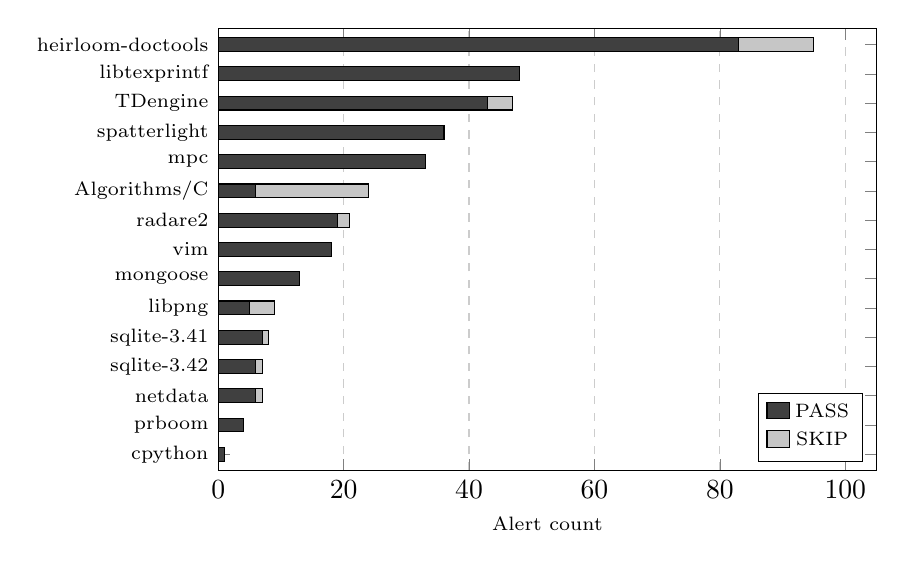
\begin{tikzpicture}
\begin{axis}[
  xbar stacked,
  bar width=5pt,
  width=0.82\columnwidth,
  height=7.2cm,
  symbolic y coords={
    cpython,prboom,netdata,sqlite42,sqlite41,
    libpng,mongoose,vim,radare2,algorithms,
    mpc,spatterlight,TDengine,libtexprintf,heirloom},
  ytick=data,
  yticklabels={
    cpython,prboom,netdata,sqlite-3.42,sqlite-3.41,
    libpng,mongoose,vim,radare2,Algorithms/C,
    mpc,spatterlight,TDengine,libtexprintf,heirloom-doctools},
  yticklabel style={font=\scriptsize},
  xmin=0, xmax=105,
  xlabel={\scriptsize Alert count},
  xmajorgrids=true,
  grid style={dashed, gray!40},
  enlarge y limits=0.04,
  legend style={at={(0.98,0.02)}, anchor=south east, legend columns=1,
    font=\scriptsize},
]
% PASS (dark)
\addplot[fill=black!75, draw=black] coordinates {
  (1,cpython)  (4,prboom)   (6,netdata)  (6,sqlite42)  (7,sqlite41)
  (5,libpng)   (13,mongoose)(18,vim)     (19,radare2)  (6,algorithms)
  (33,mpc)     (36,spatterlight)(43,TDengine)(48,libtexprintf)(83,heirloom)};
% SKIP (grey)
\addplot[fill=gray!45, draw=black] coordinates {
  (0,cpython)  (0,prboom)   (1,netdata)  (1,sqlite42)  (1,sqlite41)
  (4,libpng)   (0,mongoose) (0,vim)      (2,radare2)   (18,algorithms)
  (0,mpc)      (0,spatterlight)(4,TDengine)(0,libtexprintf)(12,heirloom)};
\legend{PASS, SKIP}
\end{axis}
\end{tikzpicture}
\caption{Alert distribution across all 15 repositories, sorted by total
  volume. Dark = PASS; grey = SKIP. The single FAIL (vim/INDEX\_CHECK,
  0.3\% of instances) is omitted.}
\label{fig:perrepo}
\end{figure}

\subsection{False Positives}
Zero false positives were observed across all 372 alerts. Correctness is argued
by construction for each handler (Section~\ref{sec:handlers}): every transformation
either provably preserves semantics under C standard guarantees or the handler
declines to act. This result holds without any post-hoc semantic testing because
the handlers are written to act only when correctness can be verified from the
local AST.

\subsection{Skip and Fail Analysis}
\label{subsec:skip}
Forty-three alerts were skipped across four documented causes: macro expansions the AST
cannot resolve to a rewritable token; vulnerabilities spanning function boundaries
that require interprocedural analysis; buffers that are dynamically rather than
statically sized, preventing \texttt{sizeof} from being applied; and patterns
already corrected in the repository version scanned. All 43 skips leave the
source file unchanged.

The single FAIL occurred in \texttt{vim/vim normal.c:1434}
(INDEX\_CHECK\_AFTER\_USE). The loop condition spans multiple source lines with
nested ternary operators. The handler's text-level search for the \texttt{\&\&}
expression failed to match across embedded newlines and indentation tabs. This case
identifies multi-line deeply-nested conditions as the current boundary of text-based
detection and motivates the AST-level operand-swap implementation planned for the
next handler revision.

% ── VI. Discussion ───────────────────────────────────────────────────────────

\section{Discussion}

\subsection{Design Philosophy}
SafeRepair's handlers are deliberately minimal. Each one fixes exactly what can be
confirmed wrong from the local AST and nothing more. The SuspiciousRealloc handler,
for example, preserves the original pointer on failure but does not insert a
\texttt{free()} call or an error return. The reason is that the appropriate response
to a failed realloc is application-specific: a server might log and continue, an
embedded system might abort, a library might propagate an error code. None of this
is knowable from local context. Adding a \texttt{free()} call would introduce a
dangling pointer and be wrong in at least half of cases. This same minimalism is why false positives are zero: handlers are written to be
right or silent, never to guess. Every SafeRepair patch is auditable the way a hand-written fix would be: a developer
reading the change can verify in seconds that the transformation is correct, because
the rule that produced it is explicit and inspectable.

\subsection{Relationship to Redemption}
The closest prior work is Redemption by Svoboda et al.~\cite{b2}, a rule-based
C/C++ APR tool covering CWE-476, CWE-457 and CWE-561/1164. It achieves 94.4\% on one codebase across three static analysis tools, using
a deterministic AST-guided approach that diverges from SafeRepair's on how
uncertain cases are handled.
Redemption explicitly applies repairs to probable false-positive alerts to maximise
coverage, accepting that adding a null check to a non-null pointer introduces only
a small performance cost. SafeRepair refuses to act unless the AST confirms the pattern, trading some
coverage for a stricter correctness guarantee.
The result is a coverage-versus-trust trade-off: Redemption is better suited to
bulk-triage workflows where a developer reviews every patch; SafeRepair is better
suited to CI/CD pipelines where patches apply without review.

The pattern sets are complementary with minimal overlap. Both systems address the
null-pointer family (Redemption handles the dereference side; SafeRepair handles
the missing guard side) but otherwise cover entirely different CWE classes and can
be deployed together. SafeRepair was evaluated on 15 repositories versus
Redemption's 3. Redemption acknowledges that its null-check handler uses a fixed
error-handling mechanism rather than inferring the appropriate return value;
SafeRepair's MissingNullCheck handler solves this by inspecting the enclosing
function's return type at repair time, inserting \texttt{return NULL},
\texttt{return -1} or a bare \texttt{return} as the context requires, and
skipping rather than guessing when neither applies.

\subsection{Relationship to Learning-Based APR}
VulRepair~\cite{b4} (43.7\% exact match) and VulMaster~\cite{b3} (20.3\% exact
match on 5,800 functions) show that neural models generalise across arbitrary bug
types, a strength that rule-based tools cannot match. Neural models do, however,
produce non-deterministic outputs, require training data and GPU infrastructure
and cannot formally guarantee semantic correctness of generated patches. For vulnerability classes with no concise structural rule, neural APR is the right
tool. For classes where the fix is fully determined by local AST context,
deterministic APR is faster, cheaper, auditable and provably correct.

\subsection{Limitations}
The four skip causes described in Section~\ref{subsec:skip} mark the current limits of the tool.
Interprocedural vulnerabilities and multi-line nested conditions represent the
most significant gaps and are the primary targets for future work. Macro-expansion
failures could be reduced by resolving macro definitions through libclang's
token-expansion API before attempting text rewriting. Dynamically sized buffers
require pointer-provenance analysis to recover the allocation size at the use
site, which is beyond local AST inspection. A handler that operates on AST operand
nodes directly rather than on source text would resolve the vim FAIL case and
eliminate the remaining macro-expansion failures. Pattern coverage is the other primary
avenue for future work: CWE-476 (null pointer dereference at the deref site, as
distinct from the allocation guard side) and CWE-415 (double free) both exhibit
the local structural signatures that SafeRepair's architecture is designed to
exploit. GCC compilation does not formally guarantee semantic correctness;
correctness for each handler is argued by construction in
Section~\ref{sec:handlers}, and that argument provides a stronger assurance than
an empirical zero-false-positive count alone.

% ── VII. Conclusion ───────────────────────────────────────────────────────────

\section{Conclusion}

Deterministic rule-based APR is viable at production scale for well-characterised
C memory-safety patterns, as SafeRepair's results show. Evaluated on 372 real-world
alerts across 15 repositories, it achieves 99.7\% repair accuracy with zero false
positives and no training data requirement. The right-or-silent design principle
makes SafeRepair safe for deployment in automated CI/CD pipelines, where an
incorrect automated patch is more harmful than no patch. Future work will extend
the handler set to additional CWE patterns and introduce AST-level operand
analysis to address interprocedural and multi-line cases currently skipped.

% ── References ───────────────────────────────────────────────────────────────

\begin{thebibliography}{00}

\bibitem{b1}
Y.~Hu, Z.~Li, K.~Shu, S.~Guan, D.~Zou, S.~Xu, B.~Yuan and H.~Jin,
``SoK: Automated Vulnerability Repair: Methods, Tools, and Assessments,''
\textit{arXiv preprint arXiv:2506.11697}, Jun.\ 2025.

\bibitem{b2}
D.~Svoboda, L.~Flynn, W.~Klieber, M.~Duggan, N.~Reimer and J.~Sible,
``Automated Code Repair for C/C++ Static Analysis Alerts,''
\textit{arXiv preprint arXiv:2508.02820}, Aug.\ 2025.

\bibitem{b3}
X.~Zhou, K.~Kim, B.~Xu, D.~Han and D.~Lo,
``Out of Sight, Out of Mind: Better Automatic Vulnerability Repair by Broadening
Input Ranges and Sources,''
in \textit{Proc.\ IEEE/ACM 46th Int.\ Conf.\ Software Engineering (ICSE)}, 2024,
pp.~1071--1083, doi:~10.1145/3597503.3639222.

\bibitem{b4}
M.~Fu, C.~Tantithamthavorn, T.~Le, V.~Nguyen and D.~Phung,
``VulRepair: A T5-Based Automated Software Vulnerability Repair,''
in \textit{Proc.\ 30th ACM Joint European Software Engineering Conf.\ and
Symp.\ Foundations of Software Engineering (ESEC/FSE)}, 2022,
pp.~935--947, doi:~10.1145/3540250.3549098.

\bibitem{b5}
N.~Jain, S.~Gandhi, A.~Sonwane, A.~Kanade, N.~Natarajan,
S.~Parthasarathy, S.~Rajamani and R.~Sharma,
``StaticFixer: From Static Analysis to Static Repair,''
\textit{arXiv preprint arXiv:2307.12465}, Jul.\ 2023.

\bibitem{b6}
CISA, NSA, FBI, and international partners,
``The Case for Memory Safe Roadmaps,'' Dec.\ 2023. [Online].
Available: \url{https://www.cisa.gov/sites/default/files/2023-12/The-Case-for-Memory-Safe-Roadmaps-508c.pdf}

\bibitem{b7}
MITRE Corporation,
``2023 CWE Top 25 Most Dangerous Software Weaknesses,'' Nov.\ 2023. [Online].
Available: \url{https://cwe.mitre.org/top25/archive/2023/2023_top25_list.html}

\bibitem{b8}
C.~Le~Goues, T.~Nguyen, S.~Forrest and W.~Weimer,
``GenProg: A Generic Method for Automatic Software Repair,''
\textit{IEEE Trans.\ Softw.\ Eng.}, vol.~38, no.~1, pp.~54--72, Jan.\ 2012,
doi:~10.1109/TSE.2011.104.

\bibitem{b9}
L.~Szekeres, M.~Payer, T.~Wei and D.~Song,
``SoK: Eternal War in Memory,''
in \textit{Proc.\ IEEE Symp.\ Security and Privacy (S\&P)}, 2013,
pp.~48--62.

\bibitem{b10}
K.~Liu, A.~Koyuncu, D.~Kim and T.~F.~Bissyand\'{e},
``TBar: Revisiting Template-Based Automated Program Repair,''
in \textit{Proc.\ 28th ACM SIGSOFT Int.\ Symp.\ Software Testing
and Analysis (ISSTA)}, 2019, pp.~189--200.

\bibitem{b11}
F.~Long and M.~Rinard,
``Automatic Patch Generation by Learning Correct Code,''
in \textit{Proc.\ 43rd Annu.\ ACM SIGPLAN-SIGACT Symp.\ Principles of
Programming Languages (POPL)}, 2016, pp.~298--312,
doi:~10.1145/2837614.2837617.

\end{thebibliography}

\end{document}
